\documentclass[12pt]{article}

\usepackage{amsmath,pstricks}
\usepackage[authoryear,round]{natbib}
\usepackage{hyperref}
\usepackage{Sweave}



\textwidth=6.2in
\textheight=8.5in
%\parskip=.3cm
\oddsidemargin=.1in
\evensidemargin=.1in
\headheight=-.3in

\newcommand{\scscst}{\scriptscriptstyle}
\newcommand{\scst}{\scriptstyle}


\newcommand{\Rfunction}[1]{{\texttt{#1}}}
\newcommand{\Robject}[1]{{\texttt{#1}}}
\newcommand{\Rpackage}[1]{{\textit{#1}}}
\newcommand{\Rmethod}[1]{{\texttt{#1}}}
\newcommand{\Rfunarg}[1]{{\texttt{#1}}}
\newcommand{\Rclass}[1]{{\textit{#1}}}

\textwidth=6.2in

\bibliographystyle{plainnat}

\begin{document}
%\setkeys{Gin}{width=0.55\textwidth}

\title{``NSAIDs modulate clonal evolution in Barrett's esophagus'' \\Using \Rpackage{BEClonalEvolutionNSAID} for reproducing results}
\author{Rumen Kostadinov}
\maketitle

\section{Figure 3}



\begin{Schunk}
\begin{Sinput}
> library("BEClonalEvolutionNSAID")
\end{Sinput}
\end{Schunk}

\begin{Schunk}
\begin{Sinput}
> con = connectDb(dbname = "sbep")
\end{Sinput}
\end{Schunk}


\begin{Schunk}
\begin{Soutput}
[1] "Patient 126"
[1] "Patient 294"
[1] "Patient 297"
[1] "Patient 315"
[1] "Patient 360"
[1] "Patient 388"
[1] "Patient 437"
[1] "Patient 555"
[1] "Patient 638"
[1] "Patient 652"
[1] "Patient 662"
[1] "Patient 672"
[1] "Patient 791"
[1] 0.2787203
[1] 0.03782836
[1] 0.002839879
[1] 0.09362534
[1] 0.09171611
[1] 0.01715497
[1] 0.1899201
\end{Soutput}
\end{Schunk}


\begin{figure}[t!]
  \centering
  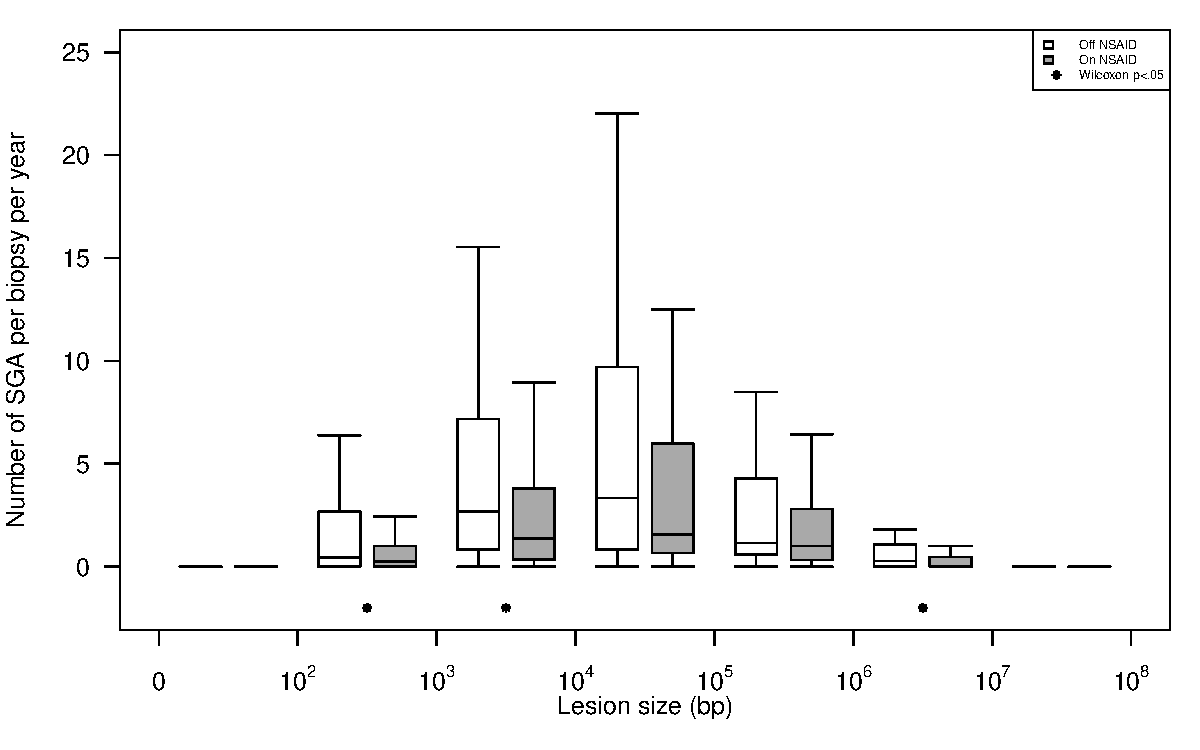
\includegraphics[width=\textwidth]{figures/guide-Figure3A.pdf}
  \caption{\label{fig:f3a} Number of newly acquired SGA events  }
\end{figure}

\begin{Schunk}
\begin{Soutput}
[1] "Patient 126"
[1] "Patient 294"
[1] "Patient 297"
[1] "Patient 315"
[1] "Patient 360"
[1] "Patient 388"
[1] "Patient 437"
[1] "Patient 555"
[1] "Patient 638"
[1] "Patient 652"
[1] "Patient 662"
[1] "Patient 672"
[1] "Patient 791"
[1] 0.0001247999
[1] 0.005664292
[1] 0.000588388
[1] 1.319588e-06
[1] 4.818289e-05
[1] 0.009581463
[1] 0.3642115
\end{Soutput}
\end{Schunk}


\begin{figure}[t!]
  \centering
  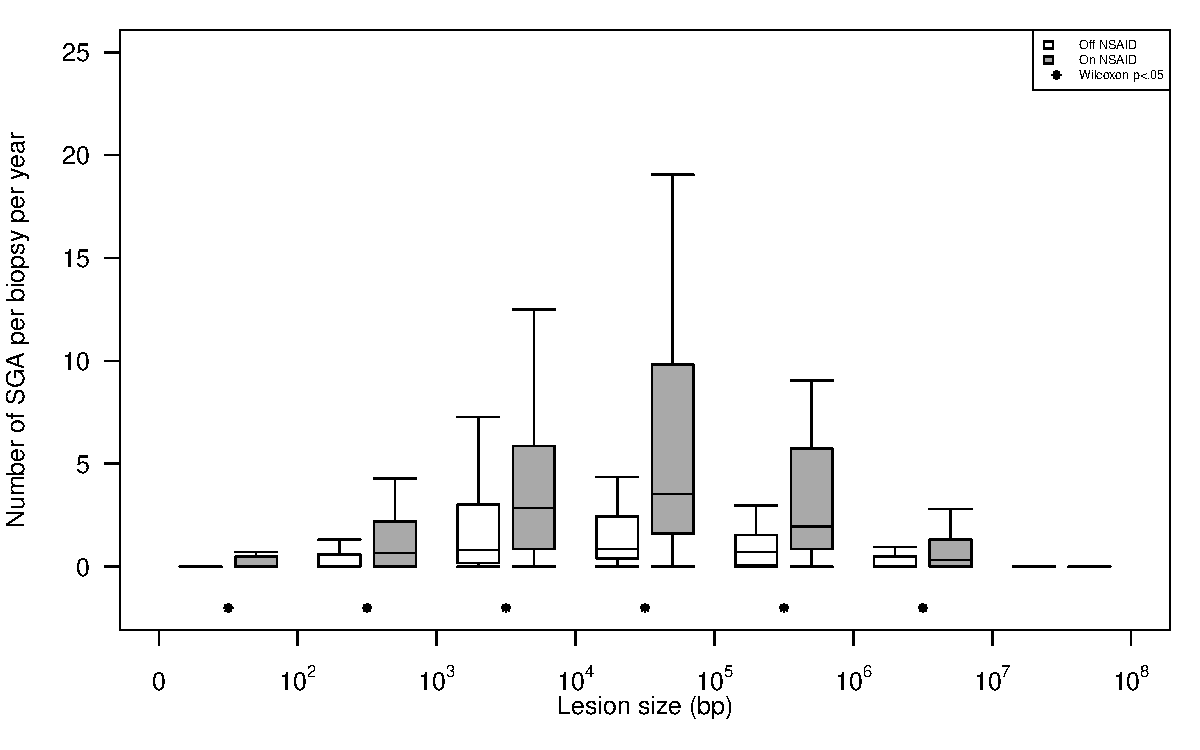
\includegraphics[width=\textwidth]{figures/guide-Figure3B.pdf}
  \caption{\label{fig:f3b} Number of regressing SGA events  }
\end{figure}


\section{System information}

This analysis was carried out on a linux machine with 12GB of RAM
using the following packages:

\begin{Schunk}
\begin{Sinput}
> sessionInfo()
\end{Sinput}
\begin{Soutput}
R version 2.12.1 (2010-12-16)
Platform: i686-pc-linux-gnu (32-bit)

locale:
 [1] LC_CTYPE=en_US.UTF-8       LC_NUMERIC=C              
 [3] LC_TIME=en_US.UTF-8        LC_COLLATE=en_US.UTF-8    
 [5] LC_MONETARY=C              LC_MESSAGES=en_US.UTF-8   
 [7] LC_PAPER=en_US.UTF-8       LC_NAME=C                 
 [9] LC_ADDRESS=C               LC_TELEPHONE=C            
[11] LC_MEASUREMENT=en_US.UTF-8 LC_IDENTIFICATION=C       

attached base packages:
[1] stats     graphics  grDevices utils     datasets  methods  
[7] base     

other attached packages:
[1] Cairo_1.5-0                  RMySQL_0.7-5                
[3] DBI_0.2-5                    BEClonalEvolutionNSAID_1.0.0
\end{Soutput}
\end{Schunk}

\end{document}
